\documentclass[
	12pt,				         				% tamanho da fonte
	openany,			     				% openright - capítulos começam em pág ímpar (insere página vazia caso preciso)
	chapter=TITLE,   				% títulos de capítulos convertidos em letras maiúsculas
	sumario=abnt-6027-2012, %tradicional, 
	oneside,			        				% twoside para impressão em verso e anverso. Oposto a oneside
	a4paper,			    				% tamanho do papel. 
	english,		         					% idioma adicional para hifenização
	brazil				        				% o último idioma é o principal do documento
	]{abntex2}

% Pacotes básicos 
\usepackage{lmodern}			% Usa a fonte Latin Modern			
\usepackage[T1]{fontenc}		% Selecao de codigos de fonte.
\usepackage[utf8]{inputenc}		% Codificacao do documento (conversão automática dos acentos)
\usepackage{lastpage}			% Usado pela Ficha catalográfica
\usepackage{indentfirst}		% Indenta o primeiro parágrafo de cada seção.
\usepackage{color}				% Controle das cores
\usepackage{graphicx}			% Inclusão de gráficos
\usepackage{microtype} 			% para melhorias de justificação
\usepackage{unijui}
\usepackage{enumitem}
\usepackage{tocloft}
 
\setlength{\cftsectionindent}{20mm}
\setlength{\cftsectionnumwidth}{10mm} 
\setlength{\cftsubsectionindent}{30mm}
\setlength{\cftsubsectionnumwidth}{10mm}

% Pacotes adicionais, usados apenas no âmbito do Modelo Canônico do abnteX2
\usepackage{lipsum}				% para geração de dummy text

% Pacotes de citações
\usepackage[brazilian,hyperpageref]{backref}	 % Paginas com as citações na bibl
\usepackage[alf]{abntex2cite}	% Citações padrão ABNT

% CONFIGURAÇÕES DE PACOTES

% Configurações do pacote backref
% Usado sem a opção hyperpageref de backref
\renewcommand{\backrefpagesname}{Citado na(s) página(s):~}
% Texto padrão antes do número das páginas
\renewcommand{\backref}{}
% Define os textos da citação
\renewcommand*{\backrefalt}[4]{
	\ifcase #1 %
		Nenhuma citação no texto.%
	\or
		Citado na página #2.%
	\else
		Citado #1 vezes nas páginas #2.%
	\fi}%

% Informações de dados para capa:
\titulo{TÍTULO DO PROJETO}
\autor{NOME DO AUTOR}
\local{Ijuí, RS, Brasil}
\data{2016}
\orientador{NOME DO ORIENTADOR}
\coorientador{NOME DO COORIENTADOR}
\tipotrabalho{Projeto de Dissertação}
\instituicao{
  Universidade Regional do Noroeste do \\Estado do Rio Grande do Sul -- UNIJUÍ
	
	Grupo de Pesquisa em Computação Aplicada (GCA)
  \par
}

% Configurações de aparência do PDF final
% alterando o aspecto da cor azul
\definecolor{blue}{RGB}{41,5,195}

% informações do PDF
\makeatletter
\hypersetup{
     	%pagebackref=true,
		pdftitle={\@title}, 
		pdfauthor={\@author},
    	pdfsubject={\imprimirpreambulo},
	    pdfcreator={LaTeX with abnTeX2},
		pdfkeywords={abnt}{latex}{abntex}{abntex2}{trabalho acadêmico}, 
		colorlinks=true,       		% false: boxed links; true: colored links
    	linkcolor=blue,          	% color of internal links
    	citecolor=blue,        		% color of links to bibliography
    	filecolor=magenta,      		% color of file links
		urlcolor=blue,
		bookmarksdepth=4
}
\makeatother
 
% Espaçamentos entre linhas e parágrafos 
% O tamanho do parágrafo é dado por:
\setlength{\parindent}{1.3cm}

% Controle do espaçamento entre um parágrafo e outro:
\setlength{\parskip}{0.2cm}  % tente também \onelineskip

% compila o indice
\makeindex
% ---

% Início do documento
\begin{document}

% Retira espaço extra obsoleto entre as frases.
\frenchspacing 

% Capa
\imprimircapa

% Resumo em português:
\setlength{\absparsep}{18pt} % ajusta o espaçamento dos parágrafos do resumo
\begin{resumo}
\label{sec:resumo}

Insira aqui o texto do resumo em português.

\textbf{Palavras-chaves}: Insira aqui as palavras-chave em português.
\end{resumo}

% Resumo em inglês:
\begin{resumo}[Abstract]
 \begin{otherlanguage*}{english}
\label{sec:abstract}

Insira aqui o texto do resumo em inglês.

\textbf{Key-words}: Insira aqui as palavras-chave em inglês.
 \end{otherlanguage*}
\end{resumo}

% Sumário:
\pdfbookmark[0]{\contentsname}{toc}
\tableofcontents*
\cleardoublepage

\textual

% Introdução:
\chapter{INTRODUÇÃO}
%Introdução
This proposal presents the plan of work to the development of the thesis of doctoral of the Postgraduate Program in Mathematical Modelling, from the Unijuí University. The research is being carried out in the the Applied Computing Research Group (GCA), which is comprised of undergraduate, master and doctoral students and professors of Unijuí University, with the collaboration of others institutions. This research is supported by the Brazilian Coordination for the Improvement of Higher Education Personnel (CAPES/PROSUP).

Next, they are presenting the context of the field of study of enterprise application integration and cloud computing, the problem that motivates this research, the objectives pursued, our contributions to date and the important collaborations that this research has received. The following sections seek to provide detailed information about the research being developed over 48 months.
% \section{Identification}
% \begin{description} 
% \item [Nome:] Daniela Freire Sellaro
% \item [Thesis supervisor:] Dr. Rafael Zancan Frantz
% \item [Affiliation of supervisor] Department of Exact Sciences and Engineering of Unijuí University - Brazil.
% \item [Joint supervisor:] Dr. Inmaculada Hernández Salmerón
% \item [Affiliation of joint supervisor] Department of Languages and Information Systems of the University of Seville - Spain
% \item [Research line:] Computational modelling, optimization and systems control
% \end{description}
%**********************************************************************************************************************************
\section{Research Context}

%-- Context
\noindent 
Companies often need to use their software ecosystems~\cite{messerschmitt:2005} to support and improve their business processes. These ecosystems are composed of many applications, usually designed without taking into account their possible integration. Within the area of Software Engineering, the field of studies known as Enterprise Integration Applications (EAI)~\cite{frantz2016} seek to provide methodologies, techniques and tools for the design and implementation of integration solutions. In general terms, an integration solution aims to orchestrate a set of applications to keep them synchronized or provide new features that can be built from those already developed. An integration solution is composed of processes that contain the integration logic and ports that encapsulate adapters for communication protocols, which connect ecosystem processes or applications to the integration solution.

Integration platforms are specialised software tools that provide support to design, implement, run, and monitor integration solution. 
In the last years, many integration platforms have been created by the EAI community. These platforms have been heavily influenced by the catalogue of conceptual integration standards documented by Hohpe and Woolf~\cite{hohpe2004} and adopt the architectural style of pipes-and-filters~\cite{alexander1977}. In an integration solution, pipes represent message channels, and filters represent atomic tasks that implement a concrete integration pattern to process encapsulated data in messages. The adoption of this architecture allows to unsynchronised the tasks that make up the integration solution.

There are several open source platforms that can be used to build integration solutions such as Mule~\cite{dossot2014}, Camel~\cite{isen2010}, Spring Integration~\cite{fisher2012}, Synapse~\cite{rademakers2008,jayasinghe2011}, Fuse~\cite{russell2012}, ServiceMix~\cite{konsek2013}, Petals~\cite{surhone2010}, Jitterbit~\cite{russell2012_1}, WSO2 ESB~\cite{indrasiri2016} and Guaraná~\cite{frantz2012}. Usually, these integration platforms provide a domain-specific language, development toolkit, test environment, monitoring tool, and runtime system. The domain-specific language is focused on the elaboration of conceptual models for the integration solution, with a level of abstraction close to the domain of the problem. The development kit is a set of software tools that allows the implementation of the solution, that is, the transformation of the conceptual model to the executable code. The testing environment allows testing individual parts or the entire integration solution, with the aim of identifying and eliminating possible defects in the implementation of the same. The monitoring tool is used to monitor, at runtime, the operation of the integration solution and detect errors that may occur during message processing. The runtime system provides all the support required to run these integration solutions.

Cloud Computing~\cite{NIST:2011} is another field of studies that has drawn the attention of the scientific community and represents a new paradigm of development, commercialization and use of software. This field has been transforming the current software ecosystems and revolutionizing the way companies provide computer support to their business processes. Cloud computing enables companies to contract service packages by dramatically reducing their total cost of ownership (TCO) with the information technology (IT) infrastructure, without sacrificing the quality of the IT support provided to their business processes. This is due mainly to the pay-as-you-go charging model that allows users to rate cloud computing based on the amount of computing resources consumed~\cite{buyya:2009,SOUSA:2009}. Along with the pay-as-you-go model, cloud computing has also brought the elasticity feature, which allows for incremental and decreasing computational resources to better meet the demands of applications running on the cloud infrastructure~\cite{DIAS:2015}.
The advancement of cloud computing technologies has led companies to a major transformation in their software ecosystem, which now includes on-premise applications, migrated applications for virtual machines in the cloud, social media applications and many other software services available in the cloud. 

% %-- Our solution
This research proposal presents the properties study that can have an impact on the performance of runtime system, regarding the ability to process messages efficiently and ensure a fair execution of tasks. runtime systems of popular integration platforms were evaluated regarding theses proprieties and it was observed that they are not sufficiently adapted to the context of the cloud computing. After, the research problems, that will contribute to migrate and adapt integration technologies to this context, are presented.
%**********************************************************************************************************************************
\section{Motivation}

%-- What is the problem? 
The quality of service, that integration solutions are able to achieve in terms of message processing, is directly related to the runtime system the integration platform. Typically, in order to achieve the desired quality of service with an integration solution, software engineers have increased computational resources in the server machine on which the integration platform is installed within the enterprise. This approach links the increased performance of an integration solution to the increase in financial costs required to augment the current hardware or the purchase of a new server with greater processing power that can generate the desired impact on the performance of the runtime systems, thus increasing the number of messages processed by the integration solutions.
The hiring of virtual machines in the cloud to host the integration platforms allows a reduction of the total cost of ownership for the realization of the EAI by the companies, as well as through the feature of elasticity of the cloud, a greater flexibility for the increment of computational resources.

This has led companies to want to migrate integration platforms and run their integration solutions in the cloud. The migration of integration platforms to virtual machines in the cloud has given rise to a new service model that is being referred to by the EAI community as integration Platform-as-a-Service (iPaaS)~\cite{pezzini2011}. Data from 2015 show that, together, Latin America, Central America and North America account for 67\% of the market for iPaaS integration platforms, followed by Europe, the Middle East and Africa, which together account for 22\%, and Asia and the Pacific with 11\% of this market, and these values should remain, with little oscillation, by the end of 2019~\cite{sharma2015}. The traditional market for integration platforms used on-premise registered growth of less than 10\% in 2016, while the market for iPaaS integration platforms had a 60\% expansion over the previous year, representing a global market of 700 million Dollars~\cite{guttridge2017}. As early as 2017, two out of three application integration projects are developed directly with cloud integration platforms~\cite{pezzini2015}. The investment made by companies in iPaaS integration platforms will increase by 40\% by 2019~\cite{sharma2015}, making iPaaS the preferred integration platform by companies and with annual revenue growth higher than the traditional platform market of integration used on-premise~\cite{guttridge2017,sharma2017}.

%-- % %-- Why it is a problem?
Given the high investments in iPaaS integration platforms, a research effort is needed to study and adapt these platforms to the new paradigm that represents cloud computing. In this context, the efficiency of runtime systems is fundamental since a number of computing resources in the cloud follows the pay-as-you-go model, and therefore has a direct impact on the financial cost involved in executing the solutions. The higher the efficiency of runtime systems, the less computational resources will need to be contracted or consumed in order for an integration solution to achieve the expected quality of service. In this proposal, performance is defined as the ability to process more messages per unit of time, without having to increase the number of computational resources allocated to the runtime system.
%**********************************************************************************************************************************
\section{Objectives}

\subsection{Main}

Reduce the average processing time of a message through the integration process, considering concurrently the optimization of the threads needed in this process.

\subsection{Specific}

\begin{enumerate}%[label=(\alph*)]
    \item Develop of a comparison framework for integration runtime system.
    \item Develop a modelling for a runtime system more efficient.
    \item Develop a prototype for a runtime system more efficient.
	\item Minimize the following variables:
    \begin{itemize}
    	\item thread management time, in relation to the creation, destruction and context change of them;
		\item waiting time of a task in the ready queues.
		\item task processing time;
    	\item time gap between a task becomes ready to execute and its execution completion.
    \end{itemize}
	\item Maximizing the total amount of messages processed by the integration process per time unit.
		\item Avoid thread concentration in the initial tasks of the integration flow in the task queue when there is an increase in the incoming message load.
	\end{enumerate}
    
%***********************************************************************************************************************************
\section{Contributions}
\label{sec:contributions}  
\noindent

This section brings the main contributions to date. 
     
\subsubsection*{Articles submitted to international journal:}

\begin{itemize}
\item \textit{Towards a Methodology to Compare Enterprise Application Integration Platforms Focusing on Performance.}

At: Software Practice and Experience. Qualis: A2. JCR: 1.60;
\item \textit{A Survey on the Runtime Systems of Enterprise Application Integration Platforms Focusing on Performance.}

At: Journal of Systems and Software. Qualis: A2. JCR: 2.44;
\item \textit{Optimization of the size of thread pool in runtime systems to Enterprise Application Integration - a mathematical modelling.}

At: Computational and Applied Mathematics. Qualis: B1. JCR: 0.96;
\item \textit{Novel Task Scheduling Proposal to Runtime System Integration Platforms.}

At: Journal of Systems and Software. Qualis: A2. JCR: 2.44
\end{itemize}

\subsubsection*{Articles presented in conference:}
\begin{itemize}
\item \textit{Task Scheduling Optimization on Enterprise Application Integration Platforms Based on the Meta-heuristic Particle Swarm Optimization}

At: XXXI Simpósio Brasileiro de Engenharia de Software (SBES) Qualis: B2.
\end{itemize}

\subsubsection*{Articles published in workshops:}

\begin{itemize}
\item \textit{Execução de Soluções de Integração de Aplicações Empresariais na Nuvem: Perspectivas e Desafios}

At: IV Seminário de Formação Científica e Tecnológica (SFCT), Ijuí, Brazil.
\end{itemize}

%**********************************************************************************************************************************
\section{Collaboration in Research}  
\label{sec:collaboration}  
\noindent

This research counts on collaborations with the following researchers:

\begin{itemize}
\item Dr. Fabricia Roos-Frantz (Unijuí University, Brazil): participation in follow-up meetings and seminars, feedbacks about our inferences, articles review, assistance in the field of study of scientific methodology and software engineering.
\item Dr. Sandro Sawicki (Unijuí University, Brazil): participation in follow-up meetings and seminars, feedbacks about our inferences, articles review, help in the field of study of optimization techniques.
\item Dr. Vitor Manuel Basto Fernandes (University Institute of Lisbon, Portugal): participation in follow-up meetings and seminars, feedbacks about our inferences, articles review, help in the field of study of data science.
\item Dr. Inmaculada Hernández Salmerón (University of Seville, Spain): participation in follow-up meetings and seminars, articles review, feedbacks about our inferences, help in the field of study of cloud computing.
\item Dr. Rafael Corchuelo (University of Seville, Spain): planning of steps of the research, planning, definition of research problems, participation in follow-up meetings and seminars, articles review, feedbacks about our inferences.
\end{itemize}
%
% Others institutions that collaborate with GCA, by means of participation in coordinated projects, joint directions, joint publications, research visits:
% \begin{itemize}
% \item Cambridge University (United Kingdom) 
% \item Rochester Institute of Technology (United States)
% \item De Montfort University (United Kingdom) 
% \item Leiden University (Netherlands) 
% \item Federal University of Rio Grande do Sul (Brazil) 
% \item Federal University of Rio de Janeiro (Brazil).
% \end{itemize}

%**********************************************************************************************************************************

\section{Structure of this Document}  
\noindent

The rest of this proposal is organised as follows: Section~\ref{cap:methodology} presents the methodology; Section~\ref{cap:stateofart} presents the technical and scientific literature review about integration platform; Section~\ref{cap:researchproblems} lists the issues to investigated derived of the literature review; Section~\ref{cap:validation} reports how results will be judged, interpreted and validated; Section~\ref{cap:schedule} shows a time-table for achieving key objectives, plans in cases where goals are not met by specific target date and informers the current state of the research; and Section~\ref{cap:infrastructure} describes the infrastructure available to develop this research.


% Capítulo 2:
\chapter{CASO DE ESTUDO}
\label{sec:capitulo02}

Insira aqui o texto do capítulo 2.

%Exemplo de seção:

\section{Ecossistema de software}

Escreva aqui sobre o ecossistema de software.

%Exemplo de figura:

Podemos ver na figura~\ref{fig01} que...

\begin{figure}[ht]
  \centering	
	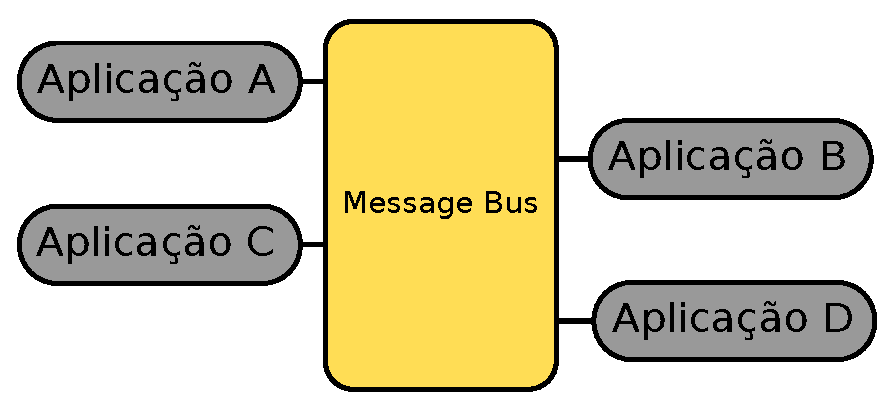
\includegraphics[scale=0.7]{figs/exemplo01.eps}
	\caption{Insira aqui o título da figura.}
	\label{fig01}
\end{figure}

%Exemplo de subseção:

\section{Modelo conceitual de integração}

Escreva aqui sobre o modelo conceitual de integração.

% Capítulo 3:
\chapter{METODOLOGIA}
\label{sec:capitulo03}

Insira aqui o texto do capítulo 3.

Podemos ver na tabela~\ref{tab01} que...

%Exemplo de tabela:

\begin{table}[h]
\centering
\vspace{0.5cm}
\begin{tabular}{r|lr}
 
Posição & País & IDH \\ 
\hline                               
1 & Noruega        & .955 \\
2 & Austrália      & .938 \\
3 & EUA            & .937 \\
4 & Holanda        & .921 \\
5 & Alemanha       & .920
 
\end{tabular}
\caption{Insira aqui o título da tabela.}
\label{tab01}
\end{table}

% Capítulo 4:
\chapter{REFERENCIAL TEÓRICO}
\label{sec:capitulo04}

Insira aqui o texto do capítulo 4.

%Exemplo de seção:

\section{Tema 1}

Escreva aqui sobre o tema 1.

%Exemplo de seção:

\section{Tema 2}

Escreva aqui sobre o tema 2.

% Capítulo 5:
\chapter{ESTÁGIO ATUAL E CRONOGRAMA DE TRABALHO}
\label{sec:capitulo05}

Insira aqui o texto do capítulo 5.

% Referências bibliográficas:
\bibliography{bibliografia}

\end{document}
